%\documentclass[draft]{beamer}
\documentclass{beamer}

\usetheme{Warsaw}
\usepackage{hyperref}


\title{Introduction to Tensor}

\author{Mingkun Yang \\
		\texttt{yangmk07@lzu.cn}}

\institute{
School of Physics\\
Lanzhou University\\
}
\date{}

\AtBeginSection[]
{
\begin{frame}<beamer>{Outline}
	\tableofcontents[currentsection]
\end{frame}
}

\begin{document}

\begin{frame}
	\titlepage
\end{frame}

\begin{frame}{Outline}
	\tableofcontents[pausesections]
\end{frame}

\section{Some Definitions}
\subsection{Basis}
\begin{frame}{Definitions Concerning Basis}
	\begin{itemize}
		\item
			Basis
			\pause
			\begin{itemize}
				\item
					Completeness
				\item
					Independence
			\end{itemize}
			\pause
		\item
			Inner Product
			\[ \langle \mathbf{r_1}, \mathbf{r_2} \rangle = \langle \sum_{i=1}^N x_1^i \mathbf{e_i}, \sum_{i=1}^N x_2^j \mathbf{e_j} \rangle =  
			\sum_{i=1}^N \sum_{j=1}^N x_1^i x_2^j \langle \mathbf{e_i}, \mathbf{e_j} \rangle = \sum_{i=1}^N \sum_{j=1}^N x_1^i x_2^j g_{ij} \]
	\end{itemize}
\end{frame}

\begin{frame}{Coordinate System}
	\pause
	\begin{itemize}
		\item
			Specail Curvilinear coordinate: Cartesain coordinate \\
			Basis: constant(fixed basis)
		\item
			General Curvilinear coordinate \\
			Basis: not constant
	\end{itemize}
\end{frame}

\subsection{Orthogonal Basis}
\begin{frame}{Orthogonal Basis}
	\begin{itemize}
		\item
			Orthogonality:
			\[ \mathbf{e_i} \cdot \mathbf{e_j} = 0 \text{  if  } i \neq j \]

			\pause
		\item
			These basis vectors are by definition the tangent vectors of the curves obtained by varying one coordinate, keeping the others fixed:
			\[ \mathbf{e_i} = \frac{\partial{\mathbf{r}}}{\partial{q^i}} \]
	\end{itemize}
\end{frame}

\begin{frame}{Visual Interpretation}
	\begin{figure}[h!]
		\centering
		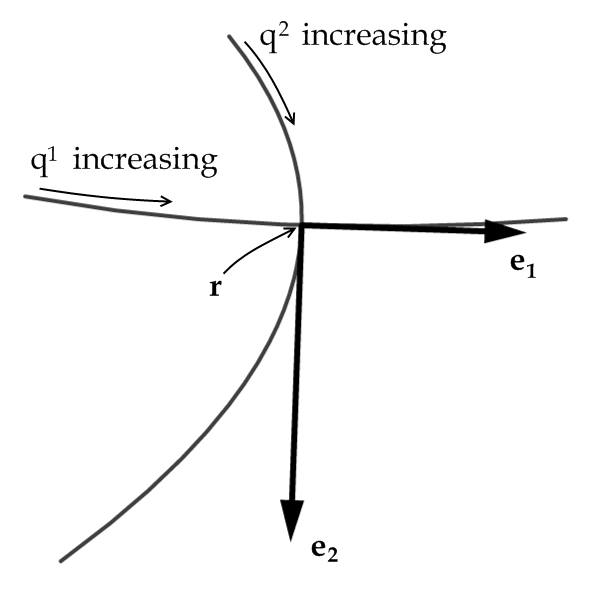
\includegraphics[scale=0.25]{OrthogonalCoordinates.png}
		\caption{\tiny Visualization of 2D orthogonal coordinates. Curves obtained by holding all but one coordinate constant are shown, along 
		with basis vectors. Note that the basis vectors aren't of equal length: they need not be, they only need to be orthogonal.}
		\centering
	\end{figure}
\end{frame}

\section{Tensors}
\begin{frame}{Tensors}
	\begin{itemize}
		\item
			Rank 0: Scalar
		\item
			Rank 1: Vector
		\item
			General Case
			\[ \displaystyle T^{i' j'} = \sum_{k,l=1}^N A^{i'}_{.k} A^{j'}_{.l} T^{kl} \]
	\end{itemize}

\end{frame}
\begin{frame}{Metric}
	\begin{definition}
		Metric(First Fundamental Form)
		\[ ds^2 = g_{ij} x^i x^j \]
		Metric Tensor
		\[ g_{ij} \equiv \langle \mathbf{e_i} \mathbf{e_j} \rangle \]
	\end{definition}
	\[ \mathbf{x_i} = g_{ij} \mathbf{x^j} \]
	\[ \mathbf{x^j} = g^{ij} \mathbf{x_i} \]
	\[ g_{ij} g^{jk} = \delta^k_i \]
\end{frame}

\section{Upstairs, Downstairs: Contravariant vs Covariant}
\begin{frame}{Common Confusion}
	\pause
	\begin{itemize}
		\item
			Contravariant or Covariant Vectors
		\item
			Contravariant or Covariant \alert{``Components''}
	\end{itemize}
	\pause
	\begin{quote}
		contravariant vectors (components) are directed \alert{parallel} to the coordinate axes, \\
		covariant vectors (components) are directed \alert{normal} (perpindicular) to constant coordinate surfaces.
	\end{quote}
\end{frame}

\begin{frame}{Special Basis}
	\pause
	\begin{itemize}
		\item
			Normalized Basis
			\[ \hat{\mathbf{e_i}} = \frac{\mathbf{e_i}}{|\mathbf{e_i}|} \]
		\item
			Covariant Basis
			\[ \mathbf{e_i} \]
		\item
			Contravariant Basis
			\[ \mathbf{e^i} \]
	\end{itemize}
\end{frame}

\begin{frame}{Special Orthogonal Basis}
	\begin{definition}[Scale factor]
		\[ h_i = | \mathbf{e_i} | \]
	\end{definition}
	\pause
	\begin{example}
		\begin{itemize}
			\item
				Polar coordinate system
				\[ h_1 = 1, h_2 = r \]
				\pause
			\item
				Spherical coordinate system
				\[ h_1 = 1, h_2 = r, h_3 = r\sin{\theta} \]
		\end{itemize}
	\end{example}
\end{frame}

\begin{frame}{Test 1}
	\[ s^2 = \sum_{i=1}^N x_i^2 = \sum_{i=1}^N x_i x^i \]

\end{frame}
\begin{frame}{Test 2}
	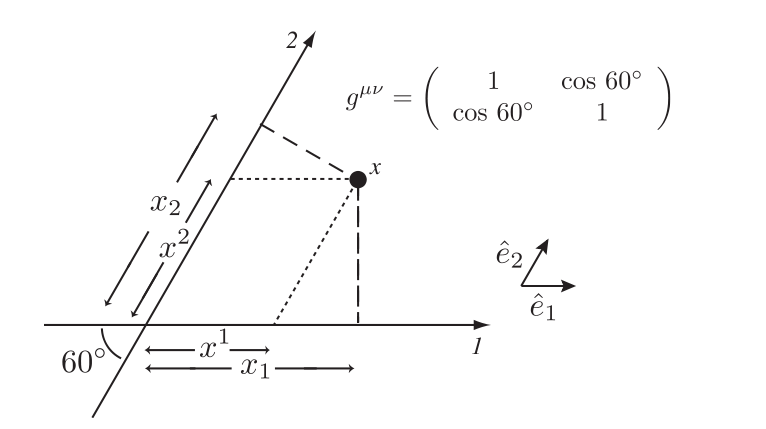
\includegraphics[scale=0.45]{ContravariantCovariant.png}
\end{frame}

\section{Mixed Tensors}
\begin{frame}{Mixed Tensors}
	Generally, a tensor with $n$ upper indices and $l$ lower indices in called a $(n,l)$ tensor.

\end{frame}

\begin{thebibliography}{9}
	\bibitem{wiki:orthogonal}
		Orthogonal coordinates \\
		\url{http://en.wikipedia.org/wiki/Orthogonal_coordinates}.
	\bibitem{AB:mpri}
		Andrew Blechman \\
		A Mathematics Primer for Physics Graduate Students.
\end{thebibliography}

\end{document}
